\subsection{Pair growth and triple intersections in the annulus}
\label{sec:annular-cap-comparison}

Keep \(r_0=\sqrt{3/2}\) and \(\rho=5/4\) as in
\cref{thm:annular-bound}. For \(r\in\{r_0,\rho\}\), write
\(B_r^{\rm vol}=\pi^2r^4/2\) for the volume of the ball and
let \(C_r(Y)\), \(P_r(Y)\) and \(H_r(Y)\) be the sums of the
volumes of single caps, pair intersections and triple
intersections, respectively, in that ball. Each cap comes
from one neighbour of \(Y\). In particular,
\(T(Y)=B_{r_0}^{\rm vol}-C_{r_0}(Y)+P_{r_0}(Y)\).

\begin{thm}[A joint bound using only single and pair caps]
\label{thm:annular-cap-comparison}
For every packing shell \(Y\) with \(2\le |y|<\sqrt6\),
\[
 P_\rho(Y)\ge \left(\frac{53}{40}\right)^3 P_{r_0}(Y),
 \qquad H_\rho(Y)\le\frac7{120}P_{r_0}(Y).
\]
Put \(\beta=(53/40)^3-1-7/120\). Then the available annular
volume from \cref{thm:annular-bound} satisfies
\begin{align}
 A(Y)&\ge B_\rho^{\rm vol}-B_{r_0}^{\rm vol}
  -\bigl(C_\rho(Y)-C_{r_0}(Y)\bigr)
  +P_\rho(Y)-\left(1+\frac7{120}\right)P_{r_0}(Y),
  \label{eq:annular-cap-exact-pairs}\\
 A(Y)&\ge B_\rho^{\rm vol}-B_{r_0}^{\rm vol}
  -\bigl(C_\rho(Y)-C_{r_0}(Y)\bigr)+\beta P_{r_0}(Y).
  \label{eq:annular-cap-one-pair}
\end{align}
Either right-hand side, denoted \(L(Y)\), gives
\(\vol V_0\ge T(Y)+(77/100)L(Y)+g(\rho)\) for every extension
of the shell. This criterion allows every angular configuration
of \(Y\).
\end{thm}

\begin{proof}
\emph{Growth of a pair intersection.}
Use unit normals \(u,v\) and plane distances \(h,k\) for the
two caps. The case of zero volume at \(r_0\) is immediate.
The closest point \(x_*\) of the intersection of the two outer
half-spaces lies on both bounding planes. Indeed, the inner
product of the normals is at most \(2/3\) by the packing
inequality, and neither point \(hu\) nor \(kv\) can be in both
half-spaces since \((2/3)\sqrt{3/2}<1\). The normals are
independent whenever the intersection has positive volume.

Let \(s=|x_*|\), \(D=r_0^2-s^2>0\), and \(H=\max(h,k)\).
The point \(x_*\) is at distance \(s\) from \(0,2hu,2kv\).
The sum of the three squared pair distances is at least
\(4(2+H^2)\) and at most \(9s^2\) by the centroid identity.
Consequently \(s^2\ge4/3\), so \(D\le1/6\), and
\[
 \mu^2:=s^2-H^2\ge 2-\frac54s^2=\frac18+\frac54D .
\]
Write \(x=x_*+p+w\), with \(p\in\operatorname{span}(u,v)\)
and \(w\) perpendicular to this span. The two half-spaces
require \(p\cdot u,p\cdot v\ge0\). The two unit rays bounding
this planar wedge have inner products \(\sqrt{s^2-h^2}\) and
\(\sqrt{s^2-k^2}\) with \(x_*\). Thus \(x_*\cdot p\ge\mu|p|\),
by expressing \(p\) as a nonnegative combination of the rays.
For \(x\) inside the ball of radius \(r_0\),
\[
 2\mu|p|+|p|^2\le D,\qquad
 \frac{|p|^2}{D}\le
 \frac{\sqrt{1+D/\mu^2}-1}{\sqrt{1+D/\mu^2}+1}<\frac19.
\]
The last comparison uses \(D/\mu^2\le1/2\) and
\(\sqrt{3/2}<5/4\).

With \(l=53/40\), the affine map
\[
 x_*+p+w\ \longmapsto\ x_*+lp+\sqrt l\,w
\]
preserves both outer half-spaces. The increase in squared
norm from \(s^2\) at the image point is at most
\[
 lD+(l^2-l)|p|^2
 \le \frac{l^2+8l}{9}D
 \le\frac{11}{8}D\le D+\frac1{16}.
\]
It thus maps into the intersection at radius \(\rho\).
Its four-dimensional Jacobian is \(l^3\), since both the normal
span and its orthogonal complement are two-dimensional.
Summation over the pairs proves the first comparison.

\emph{Volume of one triple intersection.}
Suppose the three caps of \(y_1,y_2,y_3\) intersect with positive
volume in \(B_\rho\). Put \(y_0=0\) and write their six squared
edge lengths as \(4+e_{ij}\), with \(e_{ij}\ge0\), and write
\(E_*=\sum_{0\le i<j\le3}e_{ij}\). The four points lie in a
ball of radius \(\rho\) about any point of the intersection,
so \(24+E_*\le16\rho^2=25\). Let \(G\) be the Gram matrix of
\(y_1,y_2,y_3\). Relative to the matrix \(2I+2\mathbf1\mathbf1^T\),
each unit increment in an edge excess adds a matrix bounded
below by \(-I/2\). For an edge between two nonzero vertices the
increment consists of two entries \(-1/2\). For an edge from
the origin it is
\((e_i\mathbf1^T+\mathbf1 e_i^T)/2\) in coordinate vectors,
with least eigenvalue \((1-\sqrt3)/2\).
As \(E_*\le1\), the eigenvalues of \(G\) are bounded below
by \(3/2,3/2,15/2\) in increasing order. In particular
\(\sqrt{\det G}>4\).

Let \(t_i=x\cdot y_i-|y_i|^2/2\ge0\) and
\(\bar y=(y_0+y_1+y_2+y_3)/4\). The centroid identity gives
\[
 |x-\bar y|^2+\frac12\sum_{i=1}^3t_i
 = |x|^2-\frac{24+E_*}{16}\le \frac{1-E_*}{16}=:d_* .
\]
The coordinate Jacobian from the normal span to the \(t_i\)
is \(\sqrt{\det G}\).\footnote{The linear map has the rows
\(y_i^T\) expressed in an orthonormal basis of their span.
The square of its determinant is the determinant of their
Gram matrix. Its remaining coordinate is in the orthogonal
complement and is integrated separately.}
The one-dimensional fibre perpendicular to the span has
length at most \(2\sqrt{d_*-\sum t_i/2}\).
The resulting bound on the volume \(\Gamma\) of the triple is
\[
 \Gamma\le
 \frac{1}{\sqrt{\det G}}\int_0^{2d_*}
       v^2\sqrt{d_*-v/2}\,dv
 =\frac{128\,d_*^{7/2}}{105\sqrt{\det G}}
 \le\frac{32}{105}d_*^{7/2}.
\]
Here the area factor for the sum of three nonnegative
coordinates is \(v^2/2\), and the substitution
\(v=2d_*z\) gives
\(\int_0^1 z^2\sqrt{1-z}\,dz=16/105\).

\emph{Charging a triple to its three pairs.}
Fix a pair in this triple, and let \(E\) be the sum of the
three edge excesses of the triangle consisting of that pair
and \(0\). For \(E<1\), the squared radius \(s^2\) of the
triangle circumcircle is at most \(4/3+E/6\). To verify this,
write its squared lengths \(4+x,4+y,4+z\), set
\(E=x+y+z\), \(F=xy+xz+yz\), and \(J=xyz\). The circumradius
formula gives
\[
 s^2=\frac{64+16E+4F+J}{48+8E+4F-E^2}.
\]
After cross multiplication the claimed bound is
\(8E/3+4F/3+2EF/3-E^3/6-J\ge0\), which follows from
\(E\le1\) and \(J\le F\).
The circumcentre is the closest point \(x_*\) for the pair,
by the two active inequalities proved above. Thus
\(D=r_0^2-s^2\ge(1-E)/6\).

For the two centres of this pair, now use the coordinates
\(t_i=y_i\cdot(x-x_*)\) in the normal span. Write the
two-dimensional Gram matrix as \(G_2\), with diagonal
entries \(d_i=|y_i|^2\) and off-diagonal \(c=y_1\cdot y_2\).
If \(x_*=\lambda_1 y_1+\lambda_2 y_2\), then
\(\lambda_i=1/2-(c/d_i)\lambda_j\) for \(j\ne i\).
Both coefficients are positive, since \(d_i>c\).
The edge excess bounds give \(3/8\le c/d_i\le5/8\).
It follows that \(3/16\le\lambda_i\le7/16\).
The same Gram comparison as above gives \(G_2\succeq (3/2)I\).
Writing \(v=t_1+t_2\), the squared norm of the normal
projection of \(x\) is therefore at most
\[
 s^2+2\lambda\cdot t+t^TG_2^{-1}t
 \le s^2+\frac78v+\frac23v^2\le s^2+v
 \quad(0\le v\le D\le1/6).
\]
Each such \(t\) supports an orthogonal two-dimensional disk
of area at least \(\pi(D-v)\) in the pair intersection at \(r_0\).
Since \(\sqrt{\det G_2}\le(d_1+d_2)/2\le9/2\), the pair
volume \(\Pi_0\) is at least
\[
 \frac{\pi}{\sqrt{\det G_2}}\int_0^D v(D-v)\,dv
 \ge \frac{\pi D^3}{27}.
\]
Together \(d_*\le(1-E)/16\) and \(D\ge(1-E)/6\) give
\[
 \Gamma\le\frac7{200}\Pi_0 .
\]
Indeed, the ratio of the displayed upper and lower bounds
is at most
\(32\cdot27\cdot6^3/(105\cdot16^{7/2}\pi)<7/200\),
using \(\pi>314/100\) and \(\sqrt{1-E}\le1\).
At \(E=1\) the triple volume is zero.

\emph{The number of triples using a fixed pair.}
Fix that pair and let \(w\) be a possible third centre.
Write \(a=|w|^2-4\), \(b=|w-y_1|^2-4\) and
\(c'=|w-y_2|^2-4\). These are nonnegative with
\(a+b+c'\le1-E\).
The dot products of the normal projection of \(w\) with
\(y_1,y_2\), after subtracting \((d_1/2,d_2/2)\), are
\(((a-b)/2,(a-c')/2)\). They lie in the triangle
\((1-E)\operatorname{conv}\{(1/2,1/2),(-1/2,0),(0,-1/2)\}\).
For \(G_{2,0}=\left(\begin{smallmatrix}4&2\\2&4\end{smallmatrix}\right)\),
the edge differences of the unscaled triangle have squared
norm \(1/4\) in the metric \(G_{2,0}^{-1}\).
The elementary Gram increments give
\(G_2\succeq G_{2,0}-(E/2)I\succeq(1-E/4)G_{2,0}\).
Hence the normal projections of any two possible third centres
are at distance at most \(1/2\), because
\((1-E)^2/(1-E/4)\le1\).

Also \(w\cdot(y_1+y_2)\ge(7+3a)/2\) and
\(|y_1+y_2|^2\le14\).
The squared norm of the orthogonal projection of \(w\) is
therefore at most
\[
 4+a-\frac{(7+3a)^2}{56}\le\frac{29}{9}.
\]
Any two orthogonal projections must be at distance at least
\(\sqrt{4-1/4}\), by separation of the original centres.
If their directions make angle at most \(\pi/3\), then the
squared distance is at most \(29/9\). In fact, for
\(0\le r,t\le\sqrt{29/9}\), the expression \(r^2+t^2-rt\)
is at most \(29/9\) by convexity on the square.
This contradicts \(29/9<4-1/4\).
A zero projection can occur only if it is the sole one,
by the same distance bound. In the two-dimensional orthogonal
plane at most five nonzero directions can have all mutual
angles greater than \(\pi/3\).

Every triple is charged to its three pairs, and every pair has
at most five charges. The estimate \(\Gamma\le(7/200)\Pi_0\)
therefore gives \(H_\rho(Y)\le(7/120)P_{r_0}(Y)\).
Finally, four caps cannot have positive common volume in
\(B_\rho\), since the four centres and \(0\) would give five
points with sum of squared pair distances at least \(40\)
and at most \(25\rho^2<40\).
Inclusion--exclusion thus gives
\(\vol(V(Y)\cap B_\rho)=B_\rho^{\rm vol}-C_\rho(Y)+P_\rho(Y)-H_\rho(Y)\).
Subtract \(T(Y)\) and apply the two comparisons. The exterior
estimate is \cref{thm:annular-bound}.
\end{proof}

\begin{figure}[tb]
\centering
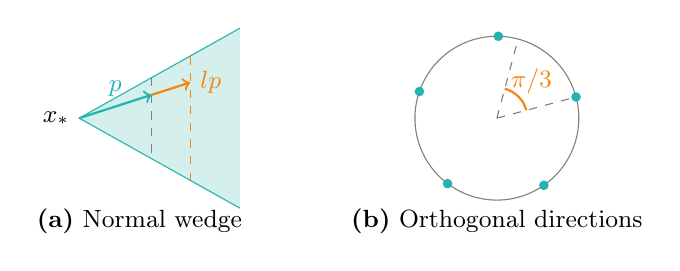
\begin{tikzpicture}[font=\small,scale=1.02]
 \begin{scope}
  \fill[TealBlue!19] (0,0)--(2,1.12)--(2,-1.12)--cycle;
  \draw[TealBlue] (2,1.12)--(0,0)--(2,-1.12);
  \draw[gray,dashed] (.9,.50)--(.9,-.50);
  \draw[BurntOrange,dashed] (1.38,.77)--(1.38,-.77);
  \draw[->,thick,TealBlue] (0,0)--(.9,.29)
      node[above,midway] {\(p\)};
  \draw[->,thick,BurntOrange] (.9,.29)--(1.38,.444)
      node[above,right] {\(lp\)};
  \node[anchor=east] at (0,0) {\(x_*\)};
  \node at (.75,-1.28) {\textbf{(a)} Normal wedge};
 \end{scope}
 \begin{scope}[xshift=5.2cm]
  \draw[gray] (0,0) circle[radius=1.02];
  \draw[gray,dashed] (0,0)--(15:1.02) (0,0)--(75:1.02);
  \draw[BurntOrange,thick] (15:.38) arc (15:75:.38);
  \node[BurntOrange] at (47:.63) {\(\pi/3\)};
  \foreach \theta in {15,89,161,233,305}{
   \fill[TealBlue] (\theta:1.02) circle[radius=1.7pt];
  }
  \node at (0,-1.28) {\textbf{(b)} Orthogonal directions};
 \end{scope}
\end{tikzpicture}
\caption{The pair comparison and the restriction on third centres.
(a) The normal wedge is invariant under \(p\mapsto lp\).
The perpendicular coordinates are stretched by \(\sqrt l\).
(b) After projecting perpendicular to the fixed pair, the angular
separation exceeds \(\pi/3\). At most five directions fit around
the circle. The drawing shows directions, so the projected
lengths need not agree.}
\label{fig:annular-cap-comparison}
\end{figure}
